\tikzset{every picture/.style={line width=0.75pt}}

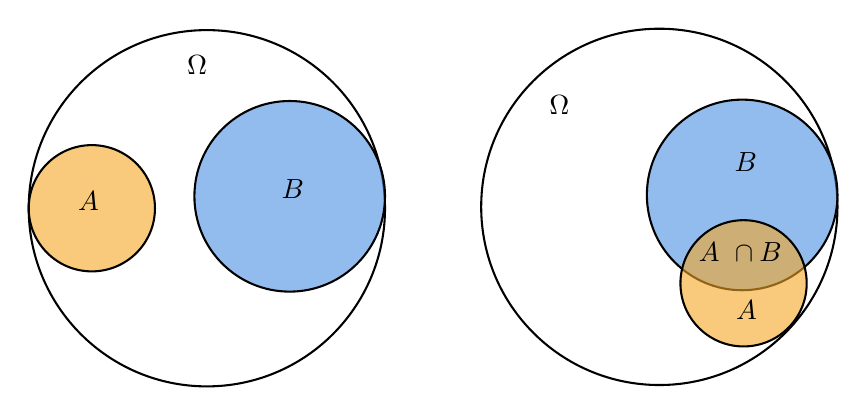
\begin{tikzpicture}[x=0.75pt,y=0.75pt,yscale=-1,xscale=1]
	
	%Shape: Circle [id:dp31605194842896434] 
	\draw   (115.67,107.5) .. controls (115.67,60.1) and (154.1,21.67) .. (201.5,21.67) .. controls (248.9,21.67) and (287.33,60.1) .. (287.33,107.5) .. controls (287.33,154.9) and (248.9,193.33) .. (201.5,193.33) .. controls (154.1,193.33) and (115.67,154.9) .. (115.67,107.5) -- cycle ;
	%Shape: Circle [id:dp9446886275503874] 
	\draw  [fill={rgb, 255:red, 245; green, 166; blue, 35 }  ,fill opacity=0.6 ] (115.67,107.5) .. controls (115.67,90.7) and (129.28,77.08) .. (146.08,77.08) .. controls (162.88,77.08) and (176.5,90.7) .. (176.5,107.5) .. controls (176.5,124.3) and (162.88,137.92) .. (146.08,137.92) .. controls (129.28,137.92) and (115.67,124.3) .. (115.67,107.5) -- cycle ;
	%Shape: Circle [id:dp36617660359881454] 
	\draw  [fill={rgb, 255:red, 74; green, 144; blue, 226 }  ,fill opacity=0.6 ] (195.5,101.75) .. controls (195.5,76.39) and (216.06,55.83) .. (241.42,55.83) .. controls (266.78,55.83) and (287.33,76.39) .. (287.33,101.75) .. controls (287.33,127.11) and (266.78,147.67) .. (241.42,147.67) .. controls (216.06,147.67) and (195.5,127.11) .. (195.5,101.75) -- cycle ;
	%Shape: Circle [id:dp6738587576196102] 
	\draw   (333.67,106.83) .. controls (333.67,59.43) and (372.1,21) .. (419.5,21) .. controls (466.9,21) and (505.33,59.43) .. (505.33,106.83) .. controls (505.33,154.24) and (466.9,192.67) .. (419.5,192.67) .. controls (372.1,192.67) and (333.67,154.24) .. (333.67,106.83) -- cycle ;
	%Shape: Circle [id:dp9633194389632203] 
	\draw  [fill={rgb, 255:red, 74; green, 144; blue, 226 }  ,fill opacity=0.6 ] (413.5,101.08) .. controls (413.5,75.72) and (434.06,55.17) .. (459.42,55.17) .. controls (484.78,55.17) and (505.33,75.72) .. (505.33,101.08) .. controls (505.33,126.44) and (484.78,147) .. (459.42,147) .. controls (434.06,147) and (413.5,126.44) .. (413.5,101.08) -- cycle ;
	%Shape: Circle [id:dp928191389662558] 
	\draw  [fill={rgb, 255:red, 245; green, 166; blue, 35 }  ,fill opacity=0.6 ] (429.67,143.67) .. controls (429.67,126.87) and (443.28,113.25) .. (460.08,113.25) .. controls (476.88,113.25) and (490.5,126.87) .. (490.5,143.67) .. controls (490.5,160.47) and (476.88,174.08) .. (460.08,174.08) .. controls (443.28,174.08) and (429.67,160.47) .. (429.67,143.67) -- cycle ;
	
	
	% Text Node
	\draw (190.5,32.5) node [anchor=north west][inner sep=0.75pt]   [align=left] {$\displaystyle \Omega $};
	% Text Node
	\draw (138,98) node [anchor=north west][inner sep=0.75pt]   [align=left] {$\displaystyle A$};
	% Text Node
	\draw (236,92) node [anchor=north west][inner sep=0.75pt]   [align=left] {$\displaystyle B$};
	% Text Node
	\draw (365,51.67) node [anchor=north west][inner sep=0.75pt]   [align=left] {$\displaystyle \Omega $};
	% Text Node
	\draw (455,150.67) node [anchor=north west][inner sep=0.75pt]   [align=left] {$\displaystyle A$};
	% Text Node
	\draw (454.33,79.33) node [anchor=north west][inner sep=0.75pt]   [align=left] {$\displaystyle B$};
	% Text Node
	\draw (437,122.67) node [anchor=north west][inner sep=0.75pt]   [align=left] {$\displaystyle A\ \cap B$};
	
	
\end{tikzpicture}